\documentclass{article}
\usepackage[utf8]{inputenc}
\usepackage{geometry}
\usepackage{graphicx}
\usepackage{amsmath}
\usepackage{amsfonts}
\usepackage{amsthm}
\usepackage{amssymb}
\usepackage[most]{tcolorbox}
\usepackage{array}
\usepackage{latexsym}
\usepackage{alltt}
\usepackage{hyperref}
\usepackage{color, colortbl}
\usepackage{float}
\usepackage{pdfpages}
\usepackage{algpseudocode}
\usepackage{multicol}
\usepackage{multirow}
\usepackage{caption}
\usepackage{xparse}
\usepackage{setspace}
\usepackage{enumitem}
\usepackage{pdflscape}
% \usepackage{parskip}
\usepackage{blindtext}
\usepackage{forest}
% \usepackage[newfloat]{minted}
\usepackage{booktabs}


\geometry
{
  a4paper,
  left=12mm,
  right=12mm,
  top=12mm,
  bottom=15mm,
}

% mybox
\newtcolorbox{mybox}[3][]
{
  colframe = #2!25,
  colback  = #2!10,
  coltitle = #2!20!black,  
  title    = {#3},
  #1,
}

\definecolor{ex}{rgb}{1.00,0.65,0.00}
\definecolor{bg}{rgb}{0.95,0.95,0.95}
% \setminted
% {
% 	mathescape=true,
% 	xleftmargin=\parindent,
% 	bgcolor=bg,
% 	escapeinside=@@
% }

% \SetupFloatingEnvironment{listing}{name=Code}

% New environments that use mybox
\newcounter{example}[section]
\newenvironment{example}[1]{\begin{mybox}[breakable]{ex}{\refstepcounter{example}\textbf{Example \thesection.\theexample #1}}}{\end{mybox}}

\newcounter{definition}[section]
\newenvironment{definition}[1]{\refstepcounter{definition}\begin{mybox}[breakable]{blue}{\textbf{Definition \thesection.\thedefinition #1}}}{\end{mybox}}

\newcounter{theorem}[section]
\newenvironment{theorem}[1]{\begin{mybox}{red}{\refstepcounter{theorem}\textbf{Theorem \thesection.\thetheorem #1}}}{\end{mybox}}

\newenvironment{formula}[1]{\begin{mybox}{cyan}{\textbf{#1}}}{\end{mybox}}

\newenvironment{practice}[1]{\begin{mybox}{ex}{\textbf{#1}}}{\end{mybox}}

% Changing maketitle
\makeatletter         
\renewcommand\maketitle{
{\raggedright % Note the extra {
\begin{center}
{\Large \bfseries \@title}\\[2ex] 
{\large \@author \ - \@date}\\[2ex]
\end{center}}} % Note the extra }
\makeatother

% \onehalfspacing % adjust spacing
\setlength{\parskip}{0.5\baselineskip}

% macros
\newcommand{\prob}[1]{\textbf{\textit{P}}\left\{#1\right\}}
\newcommand{\expc}[1]{\mathbf{E}\left(#1\right)}
\newcommand{\expcs}[1]{\mathbf{E}^2\left(#1\right)}
\newcommand{\var}[1]{\text{Var}\left( #1 \right)}
\newcommand{\ra}{\rightarrow}
\newcommand{\Ra}{\Rightarrow}
\newcommand{\R}[2]{\tikz [remember picture,overlay] \node (#1) {#2};}

\def\circtxt#1{$\mathalpha \bigcirc \mkern-13mu \mathtt #1$}
\def\smiley{\textcircled{\scriptsize $\mkern3mu\ddot{\ } \mkern-15mu \smallsmile$}}

\NewDocumentCommand{\dsum}{%
    e{^_}
}{%
  {% 
    \displaystyle\sum
    \IfValueT{#1}{^{#1}}
    \IfValueT{#2}{_{#2}}
  }
}%

% maketitle variables
\title{CENG 232 - Chapter 5: Synchronous Sequential Logic}
\author{Burak Metehan Tunçel}
\date{May 2022}

\begin{document}

\maketitle

\begin{multicols*}{2}
\setlength{\columnsep}{1.5cm}
\setlength{\columnseprule}{0.2pt}

\section{Sequential Circuits}

Figure 5.1 shows a block diagram of a sequential circuit. It consists of a combinational circuit to which memory elements are connected to form a feedback path.

\begin{figure}[H]
  \centering
  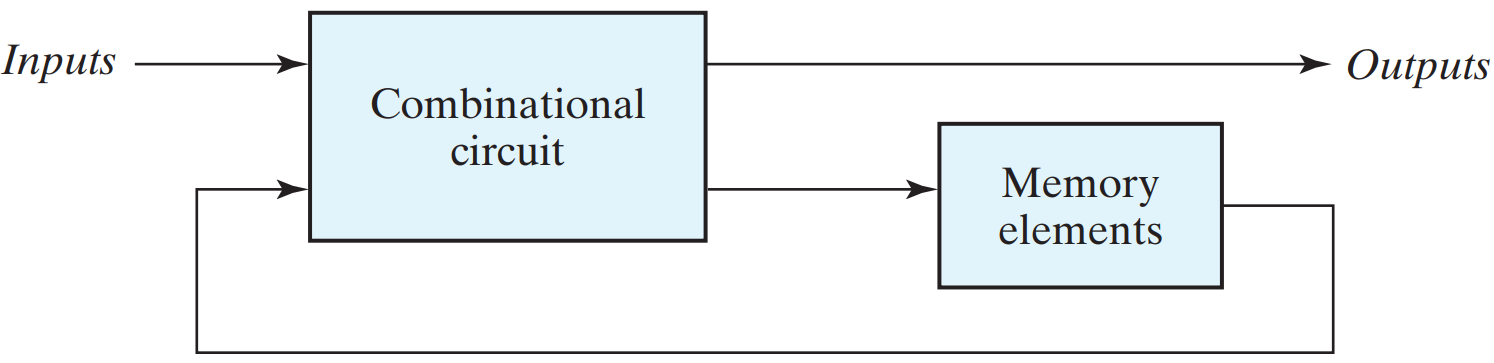
\includegraphics[width=\linewidth]{img/fig-5.1.png}
  \caption{Block diagram of sequential circuit}
  \label{fig:5.1}
\end{figure}

\textbf{A sequential circuit is specified by a time sequence of inputs, outputs, and internal states}.

There are two main types of sequential circuits, and their classification is a function of the timing of their signals:
\begin{itemize}
  \item A \textit{\textbf{synchronous} sequential circuit} is a system whose behavior can be defined from the knowledge of its signals at discrete instants of time.
  \item The behavior of an \textit{\textbf{asynchronous} sequential circuit} depends upon the input signals at any instant of  time \textit{and} the order in which the inputs change
\end{itemize}

A synchronous sequential circuit employs signals that affect the storage elements at only \textit{discrete instants of time}. Synchronization is achieved by a timing device called a \textit{clock generator}. The storage elements (memory) used in clocked sequential circuits are called \textit{flip-flops}.

The block diagram of a synchronous clocked sequential circuit is shown in 
Fig. 2.
\begin{figure}[H]
  \centering
  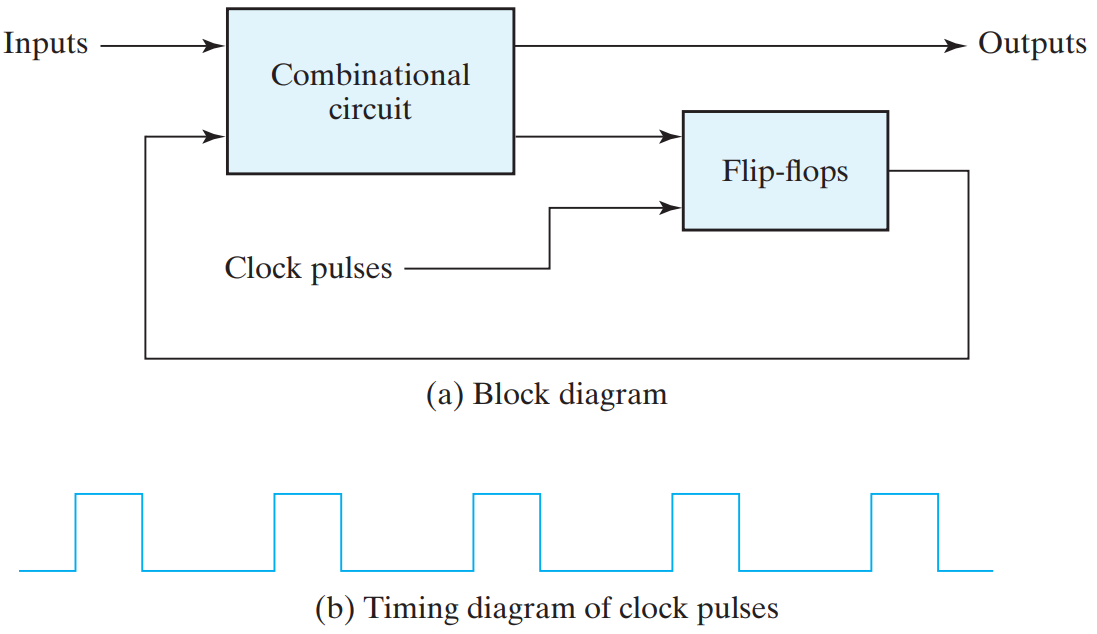
\includegraphics[width=\linewidth]{img/fig-5.2.png}
  \caption{Synchronous clocked sequential circuit}
  \label{fig:5.2}
\end{figure}

\begin{itemize}
  \item The \textit{outputs} are formed by a \textit{combinational logic function of the inputs to the circuit or the values stored in the flip-flops (or both)}. 
  \item The \textit{value that is stored in a flip-flop} when the clock pulse occurs is also determined by \textit{the inputs to the circuit or the values presently stored in the flip-flop (or both)}.
  \item The \textit{new value is stored} (i.e., the flip-flop is \textit{updated}) when a pulse of the clock signal occurs.
\end{itemize}

\textbf{Note:} The output of a combinational circuit depends on only the inputs to the circuit; the output of a sequential circuit depends on the inputs to the circuit and the present state of the storage elements.


\section{Storage Element: Latches}
\label{sec:stor-ele-latch}

A storage element in a digital circuit can maintain a binary state indefinitely (as long as power is delivered to the circuit), until directed by an input signal to switch states.

\textit{Storage elements that operate with signal levels (rather than signal transitions) are referred to as latches; those controlled by a clock transition are flip-flops}. Latches are said to be \textit{level-sensitive devices}; flip-flops are \textit{edge-sensitive devices}. The two types of storage elements are related because \textit{latches are the basic circuits from which all flip-flops are constructed}.

\subsection{SR Latch}
\label{subsec:sr-latch}

The \textit{SR} latch is a circuit with two cross-coupled NOR gates or two cross-coupled NAND gates, and two inputs labeled \textit{S} for set, and \textit{R} for reset. The \textit{SR} latch constructed with two cross-coupled NOR gates is shown in Fig. 5.3. 
\begin{figure}[H]
  \centering
  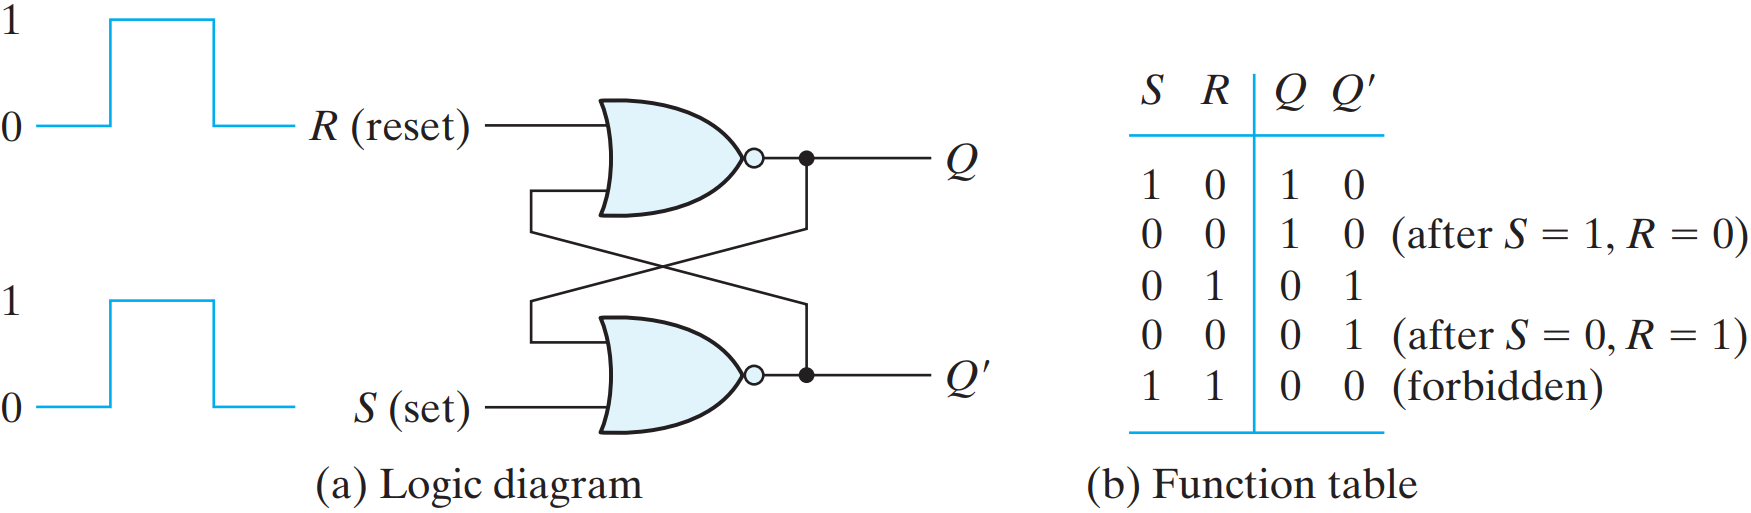
\includegraphics[width=\linewidth]{img/fig-5.3.png}
  \caption{SR latch with NOR gates}
  \label{fig:5.3}
\end{figure}
\noindent The latch has two useful states. When output $Q = 1$ and $Q' = 0$, the latch is said to be in the \textit{set} state. When $Q = 0$ and $Q' = 1$, it is in the \textit{reset} state.

However, when both inputs are equal to 1 at the same time, a condition in which both outputs are equal to 0 (rather than be mutually complementary) occurs. So, in pratice, \textbf{setting both inputs to 1 is forbidden}. Under normal conditions, both inputs of the latch remain at 0 unless the state has to be changed.

\vspace*{\fill}
\columnbreak

The \textit{SR} latch with two cross-coupled NAND gates is shown in Fig. 4. 
\begin{figure}[H]
  \centering
  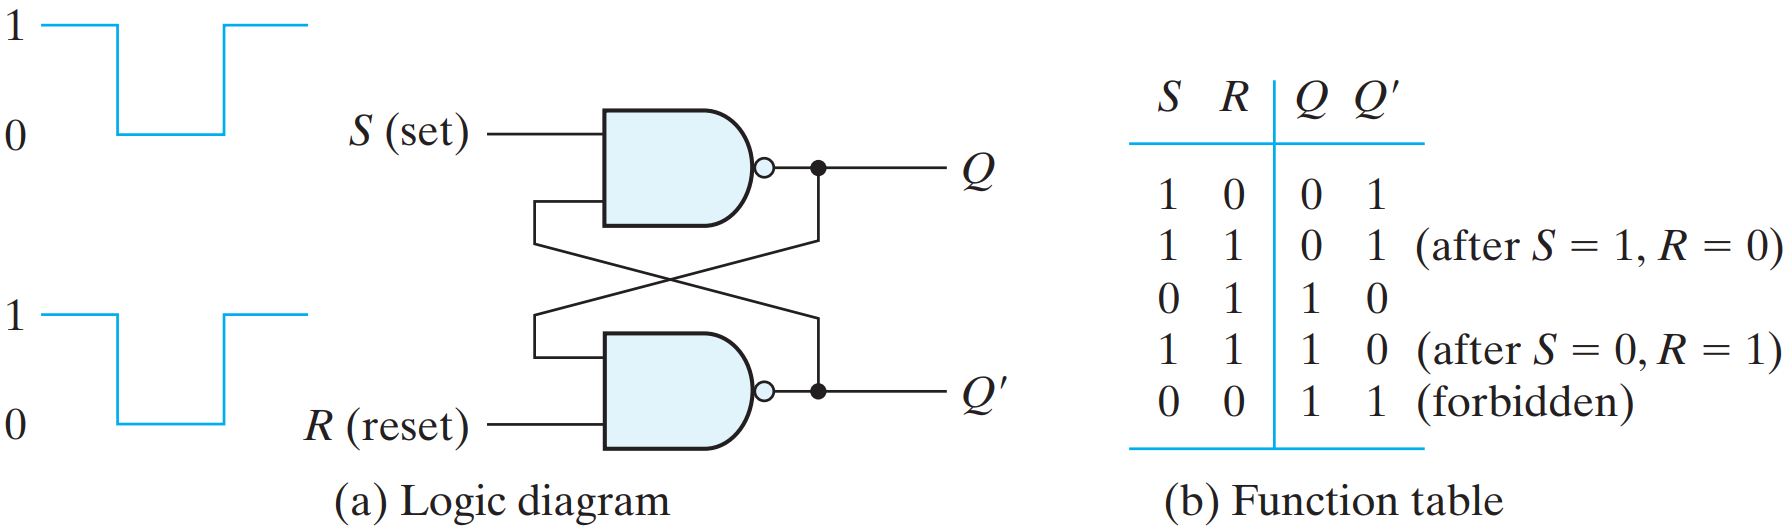
\includegraphics[width=\linewidth]{img/fig-5.4.png}
  \caption{SR latch with NAND gates}
  \label{fig:5.4}
\end{figure}
It operates with both inputs normally at 1, unless the state of the latch has to be changed. The condition that is forbidden for the NAND latch is both inputs being equal to 0 at the same time, an input combination that should be avoided.

The operation of the basic $SR$ latch can be modified by providing an additional input signal that determines (controls) when the state of the latch can be changed by determining whether $S$ and $R$ (or $S'$ and $R'$) can affect the circuit. An SR latch with a control input is shown in Fig. 5. It consists of the basic SR latch and two additional NAND gates.
\begin{figure}[H]
  \centering
  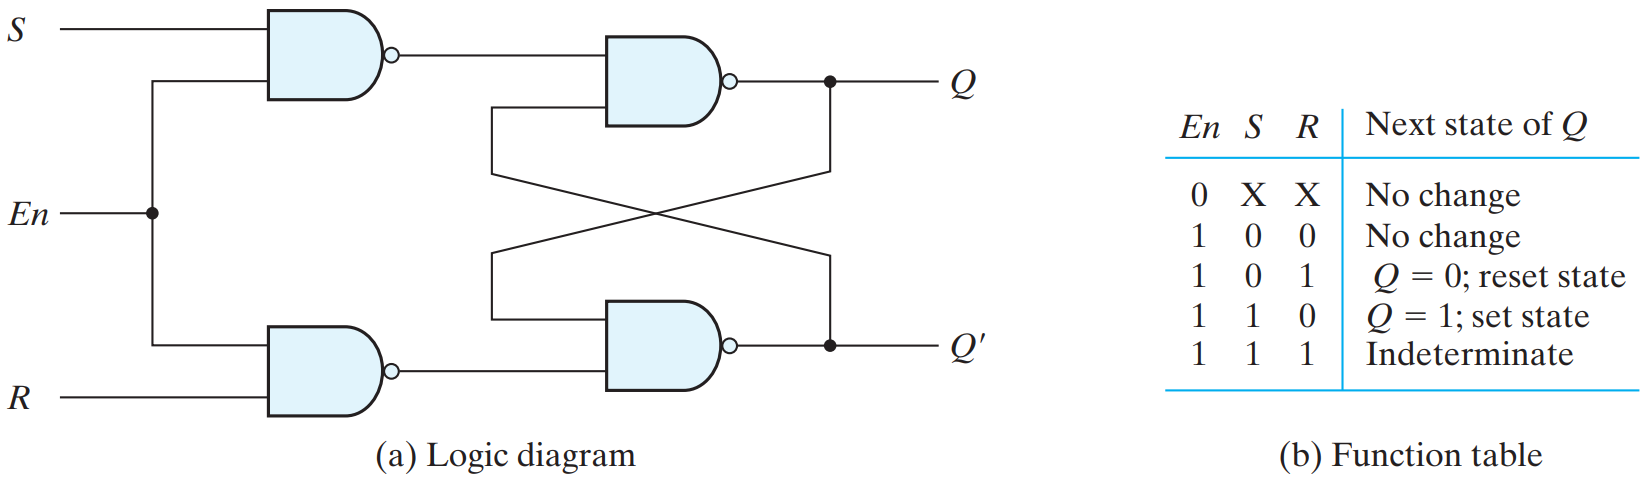
\includegraphics[width=\linewidth]{img/fig-5.5.png}
  \caption{SR latch with control input}
  \label{fig:5.5}
\end{figure}
An indeterminate condition occurs when all three inputs are equal to 1. This condition places 0's on both inputs of the basic $SR$ latch, which puts it in the undefined state.

\textbf{Note:}
\begin{itemize}[leftmargin=0.5cm]
  \item Input condition puts an $SR$ NOR latch into an indeterminate state is the condition ``Both inputs are 1''.
  \item Input condition puts an $SR$ NAND latch into an indeterminate state is the condition ``Both inputs are 0''.
\end{itemize}

\subsection{D Latch (Transparent Latch)}
\label{subsec:d-latch}

One way to eliminate the undesirable condition of the indeterminate state in the $SR$ latch is to ensure that inputs $S$ and $R$ are never equal to 1 at the same time. This is done in the $D$ latch, shown in Fig. 6. 
\begin{figure}[H]
  \centering
  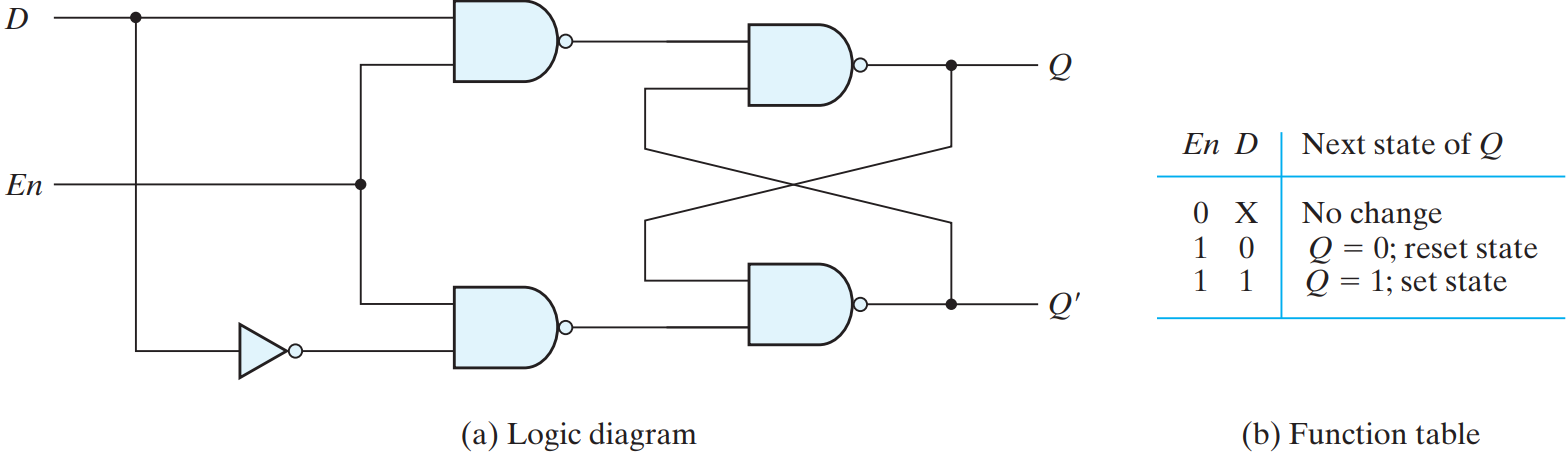
\includegraphics[width=\linewidth]{img/fig-5.6.png}
  \caption{D Latch}
  \label{fig:5.6}
\end{figure}
\noindent This latch has only two inputs: $D$ (data) and $En$ (enable). The $D$ input goes directly to the $S$ input, and its complement is applied to the $R$ input. 

The binary information present at the data input of the $D$ latch is transferred to the $Q$ output when the enable input is asserted. The output follows changes in the data input as long as the enable input is asserted.

The graphic symbols for the various latches are shown in Fig. 5.7.
\begin{figure}[H]
  \centering
  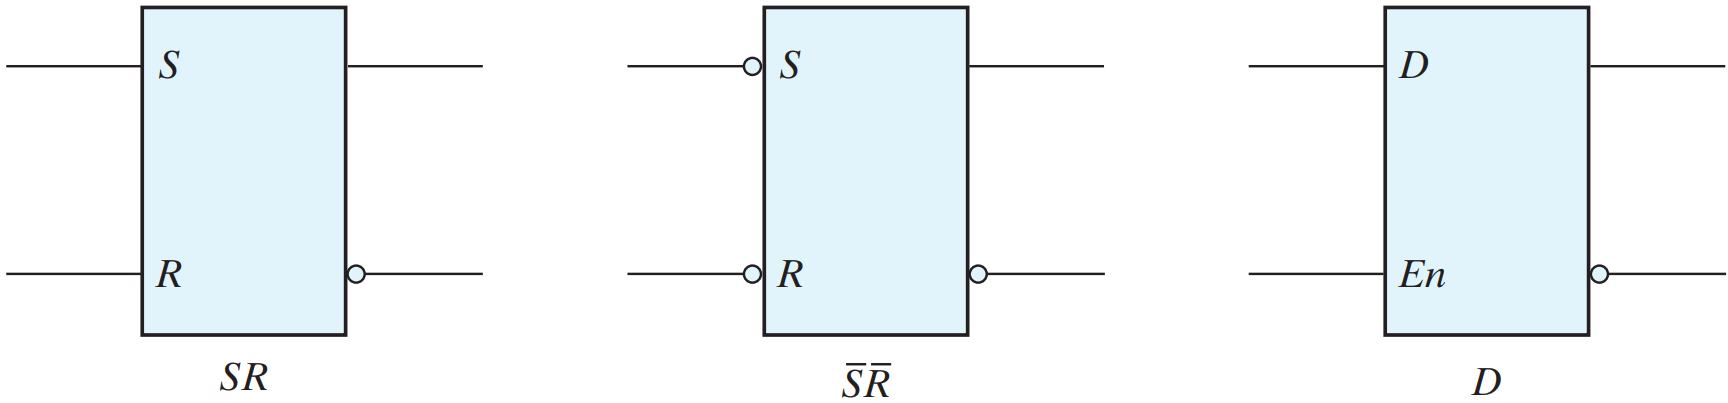
\includegraphics[width=\linewidth]{img/fig-5.7.png}
  \caption{Graphic symbols for latches}
  \label{fig:5.7}
\end{figure}

\textbf{Note:} A transparent latch has a data input, an enable input, and output. When the enable input is asserted, the output of the latch follows the input to the latch. When the enable input is de-asserted, the output of the latch is held at the value that was present at the moment the enable input was de-asserted.


\section{Storage Element: Flip-Flops}
\label{sec:stor-ele-flip-flop}

Flip-flop circuits are constructed in such a way as to make them operate properly when they are part of a sequential circuit that employs a common clock. The problem with the latch is that it responds to a change in the \textit{level} of a clock pulse. The key to the proper operation of a flip-flop is to trigger it only during a signal \textit{transition}.

\begin{figure}[H]
  \centering
  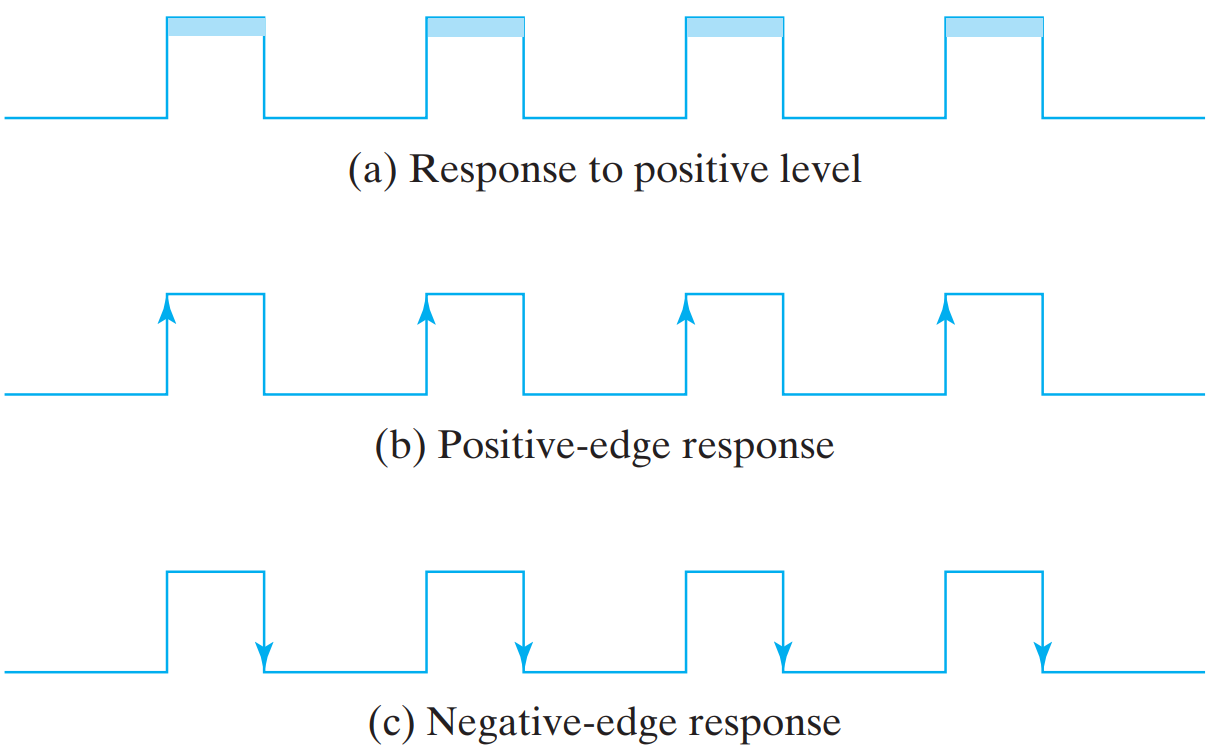
\includegraphics[width=\linewidth]{img/fig-5.8.png}
  \caption{Clock response in latch and flip-flop}
  \label{fig:5.8}
\end{figure}

There are two ways that a latch can be modified to form a flip-flop.
\begin{itemize}
  \item One way is to employ two latches in a special configuration that isolates the output of the flip-flop and prevents it from being affected while the input to the flip-flop is changing.
  \item Another way is to produce a flip-flop that triggers only during a signal transition (from 0 to 1 or from 1 to 0) of the synchronizing signal (clock) and is disabled during the rest of the clock pulse.
\end{itemize}

\subsection{Edge-Triggered D Flip-Flop}
\label{subsec:edge-trig-d-flip-flop}

The construction of a $D$ flip-flop with two $D$ latches and an inverter is shown in Fig. 9. It is often referred to as a master–slave flip-flop. The circuit samples the $D$ input and changes its output $Q$ \textit{only at the negative edge} of the synchronizing or controlling clock.
\begin{figure}[H]
  \centering
  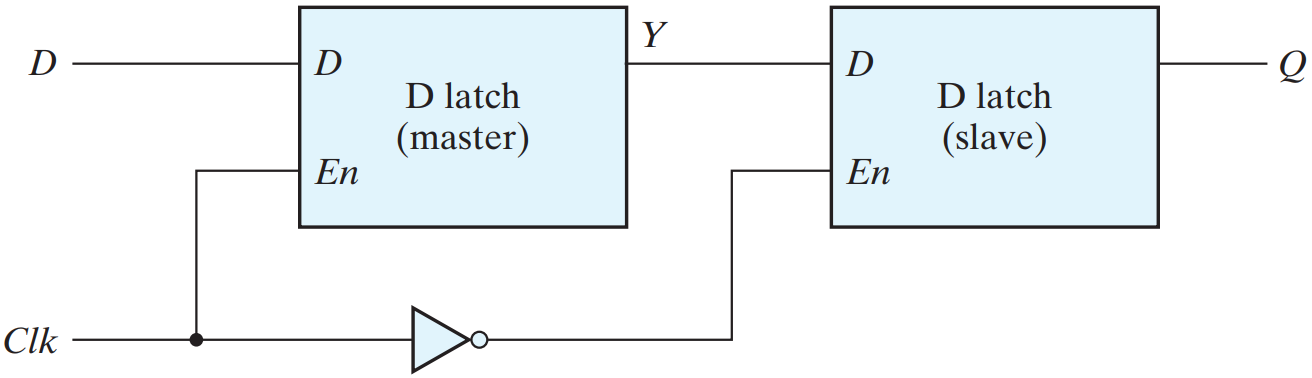
\includegraphics[width=\linewidth]{img/fig-5.9.png}
  \caption{Master–slave $D$ flip-flop}
  \label{fig:5.9}
\end{figure}
\noindent \textit{A change in the output of the flip-flop can be triggered only by and during the transition of the clock from 1 to 0}.

Another construction of an edge-triggered $D$ flip-flop uses three $SR$ latches as shown in Fig. 10.
\begin{figure}[H]
  \centering
  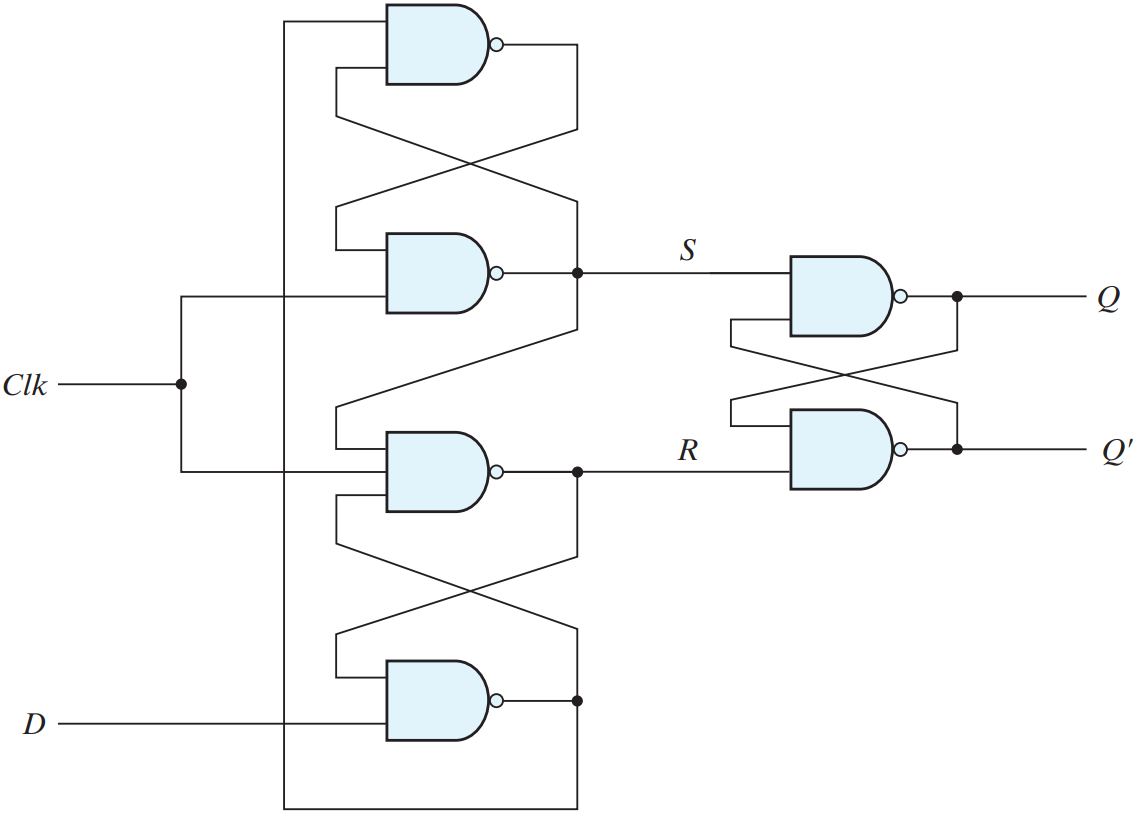
\includegraphics[width=\linewidth]{img/fig-5.10.png}
  \caption{D-type positive-edge-triggered flip-flop}
  \label{fig:5.10}
\end{figure}

The behavior of the master–slave flip-flop just described dictates that
\begin{enumerate}[leftmargin=0.5cm]
  \item The output may change only once,
  \item A change in the output is triggered by the negative edge of the clock,
  \item The change may occur only during the clock's negative level.
\end{enumerate}
\noindent The value that is produced at the output of the flip-flop is the value that was stored in the master stage immediately before the negative edge occurred. It is also possible to design the circuit so that the flip-flop output changes on the positive edge of the clock.

In sum, \textit{when the input clock in the positive-edge-triggered flip-flop makes a positive transition, the value of \textnormal{D} is transferred to \textnormal{Q}}.

The graphic symbol for the edge-triggered $D$ flip-flop is shown in Fig. 11.
\begin{figure}[H]
  \centering
  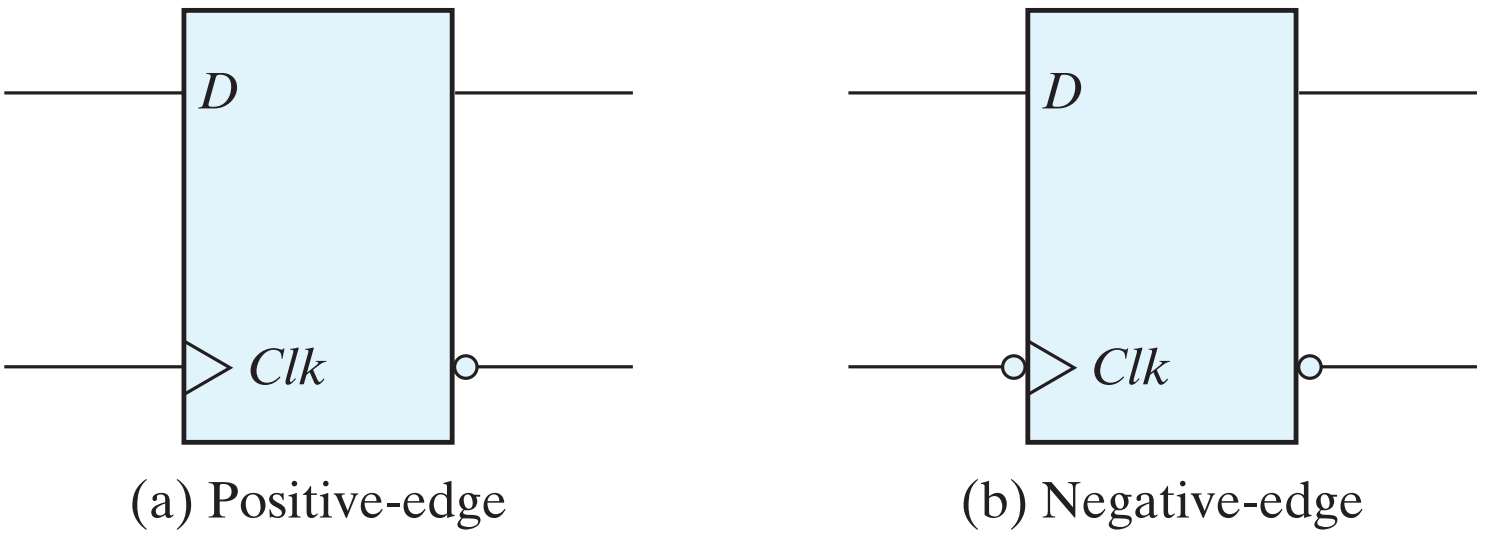
\includegraphics[width=\linewidth]{img/fig-5.11.png}
  \caption{Graphic symbol for edge-triggered D flip-flop}
  \label{fig:5.11}
\end{figure}

\textbf{Note:} A positive-edge flip-flop is one that is activated by the rising (positive) edge of the clock (synchronizing signal).

\subsection{Other Flip-Flops}
\label{subsec:other-flip-flops}

The most economical and efficient flip-flop constructed in this manner is the edge-triggered $D$ flip-flop, because it requires the smallest number of gates. Other types of flip-flops can be constructed by using the $D$ flip-flop and external logic. Two flip-flops less widely used in the design of digital systems are the $JK$ and $T$ flip-flops.

There are three operations that can be performed with a flip-flop:
\begin{enumerate}[]
  \item Set it to 1,
  \item Reset it to 0, or 
  \item Complement its output.
\noindent \end{enumerate}

\subsubsection{JK Flip-Flops}
\label{subsubsec:jk-flip-flops}

With only a single input, the $D$ flip-flop can set or reset the output. The $JK$ flip-flop has two inputs and performs all three operations. The circuit diagram of a $JK$ flip-flop constructed with a $D$ flip-flop 
and gates is shown in Fig. 12(a).
\begin{figure}[H]
  \centering
  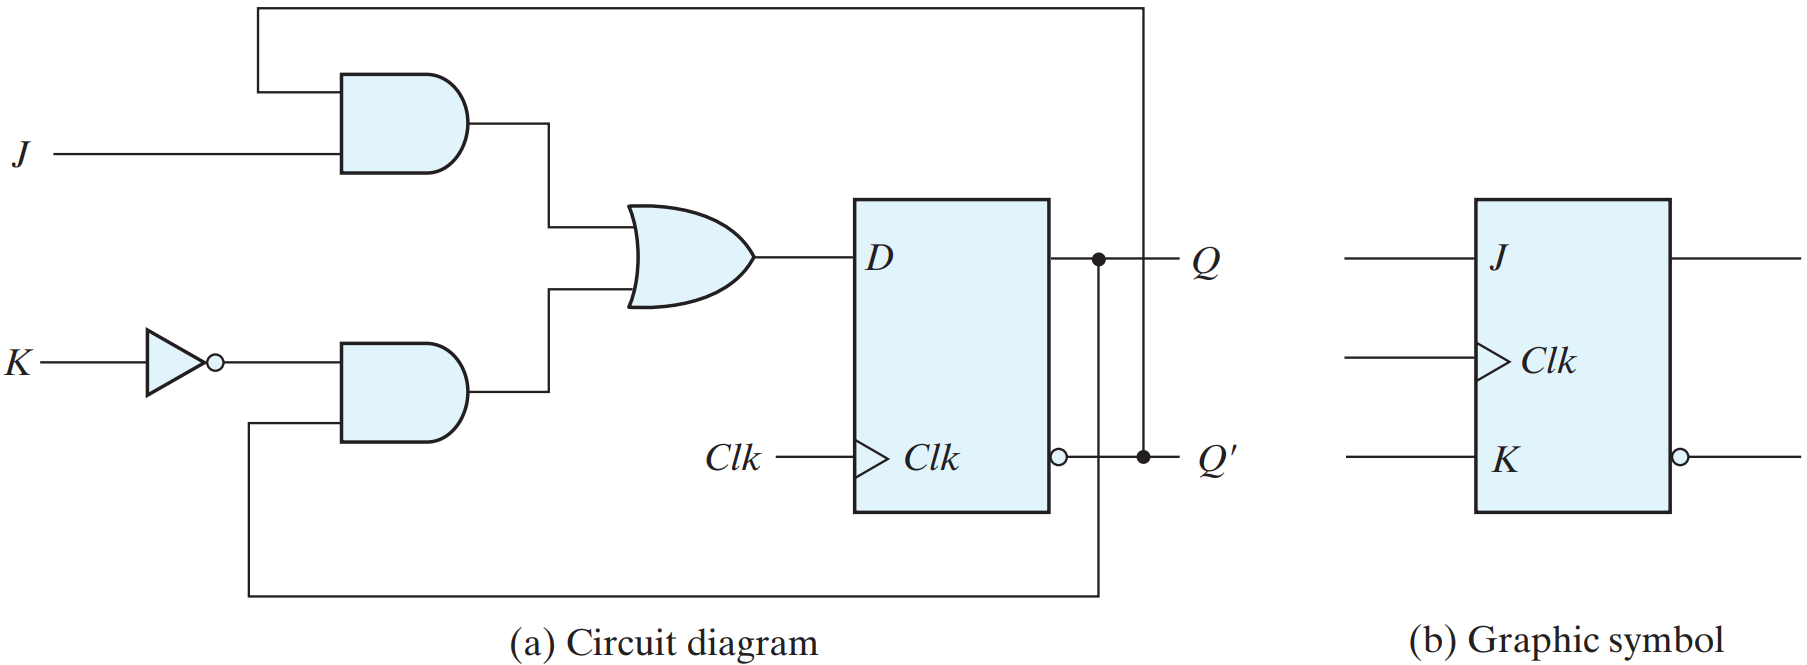
\includegraphics[width=\linewidth]{img/fig-5.12.png}
  \caption{$JK$ flip-flop}
  \label{fig:5.12}
\end{figure}
\noindent The $J$ input sets the flip-flop to 1, the $K$ input resets it 
to 0, and when both inputs are enabled, the output is complemented. This can be verified by investigating the circuit applied to the D input:
\begin{equation*}
  D = JQ' + K'Q
\end{equation*}
The graphic symbol for the $JK$ flip-flop is shown in Fig. 12(b).

\vspace*{\fill}
\columnbreak

\subsubsection{T Flip-Flops}
\label{subsubsec:t-flip-flops}

The $T$ (toggle) flip-flop is a complementing flip-flop and can be obtained from a $JK$ flip-flop when inputs $J$ and $K$ are tied together. This is shown in Fig. 13(a).
\begin{figure}[H]
  \centering
  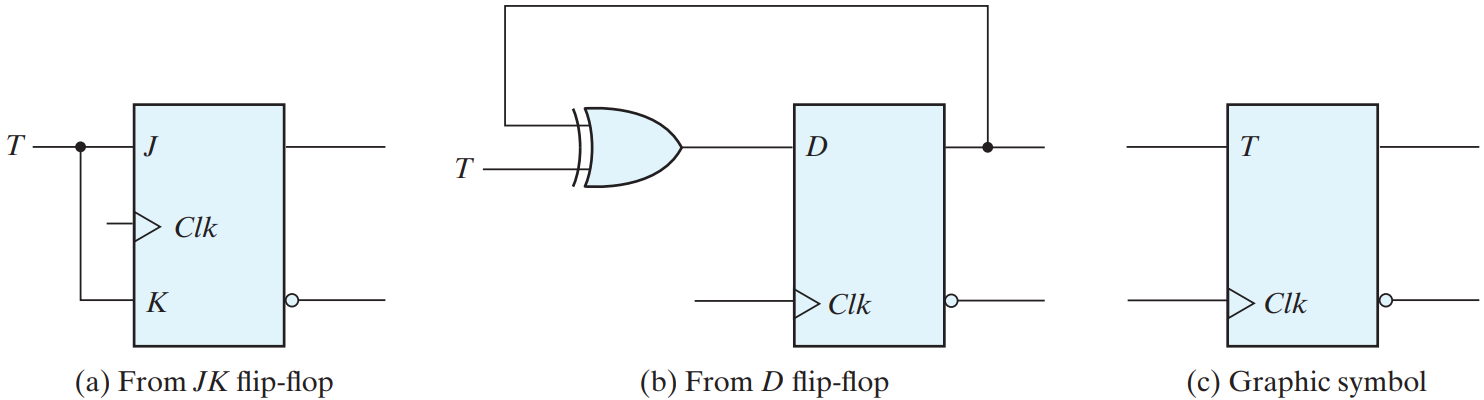
\includegraphics[width=\linewidth]{img/fig-5.13.png}
  \caption{T flip-flop}
  \label{fig:5.13}
\end{figure}
The complementing flip-flop is useful for designing binary counters. The $T$ flip-flop can be constructed with a $D$ flip-flop and an exclusive-OR gate as shown in Fig. 13(b). The expression for the D input is
\begin{equation*}
  D = T \oplus Q = TQ' + T'Q
\end{equation*}
The graphic symbol for this flip-flop has a $T$ symbol in the input.


\subsection{Characteristic Tables}
\label{subsec:char-tables}

The characteristic tables of three types of flip-flops are presented in Table 5.1.
\begin{figure}[H]
  \centering
  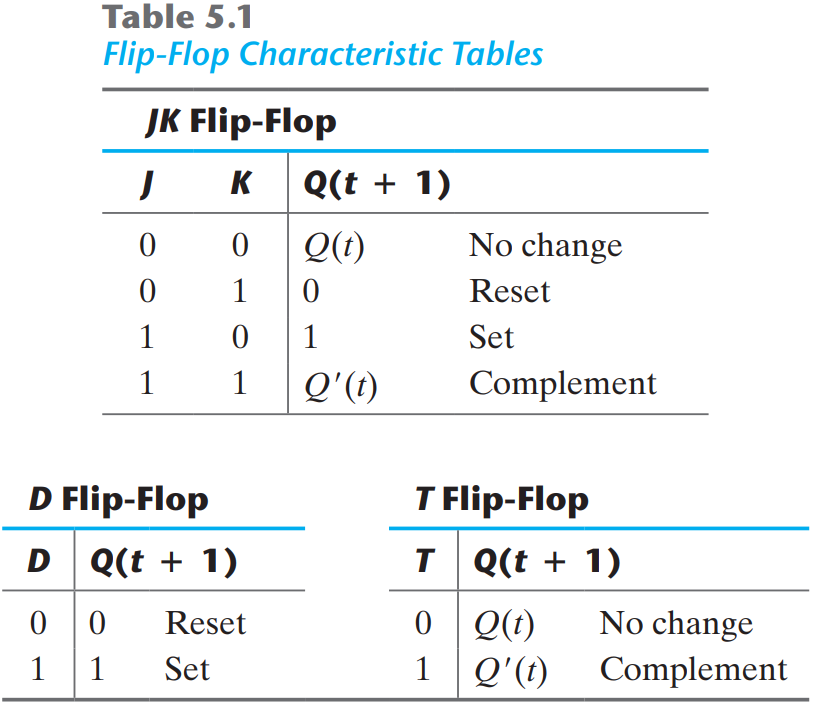
\includegraphics[width=\linewidth]{img/table-5.1.png}
  \label{table:5.1}
\end{figure}


\subsection{Characteristic Equations}
\label{subsec:char-equations}

$D$ flip-flop:
\begin{equation*}
  Q(t + 1) = D
\end{equation*}
$JK$ flip-flop:
\begin{equation*}
  Q(t + 1) = JQ' + K'Q
\end{equation*}
$T$ flip-flop:
\begin{equation*}
  Q(t + 1) = T \oplus Q = TQ' + T'Q
\end{equation*}

\setcounter{figure}{14}


\section{Analysis of Clocked Sequential Circuits}
\label{sec:analysis-clocked-seq-circ}

\subsection{State Equations}
\label{subsec:state-equations}

A \textit{state equation} (also called a \textit{transition equation}) specifies the next state as a function of the present state and inputs. Consider the sequential circuit shown in Fig. 15
\begin{figure}[H]
  \centering
  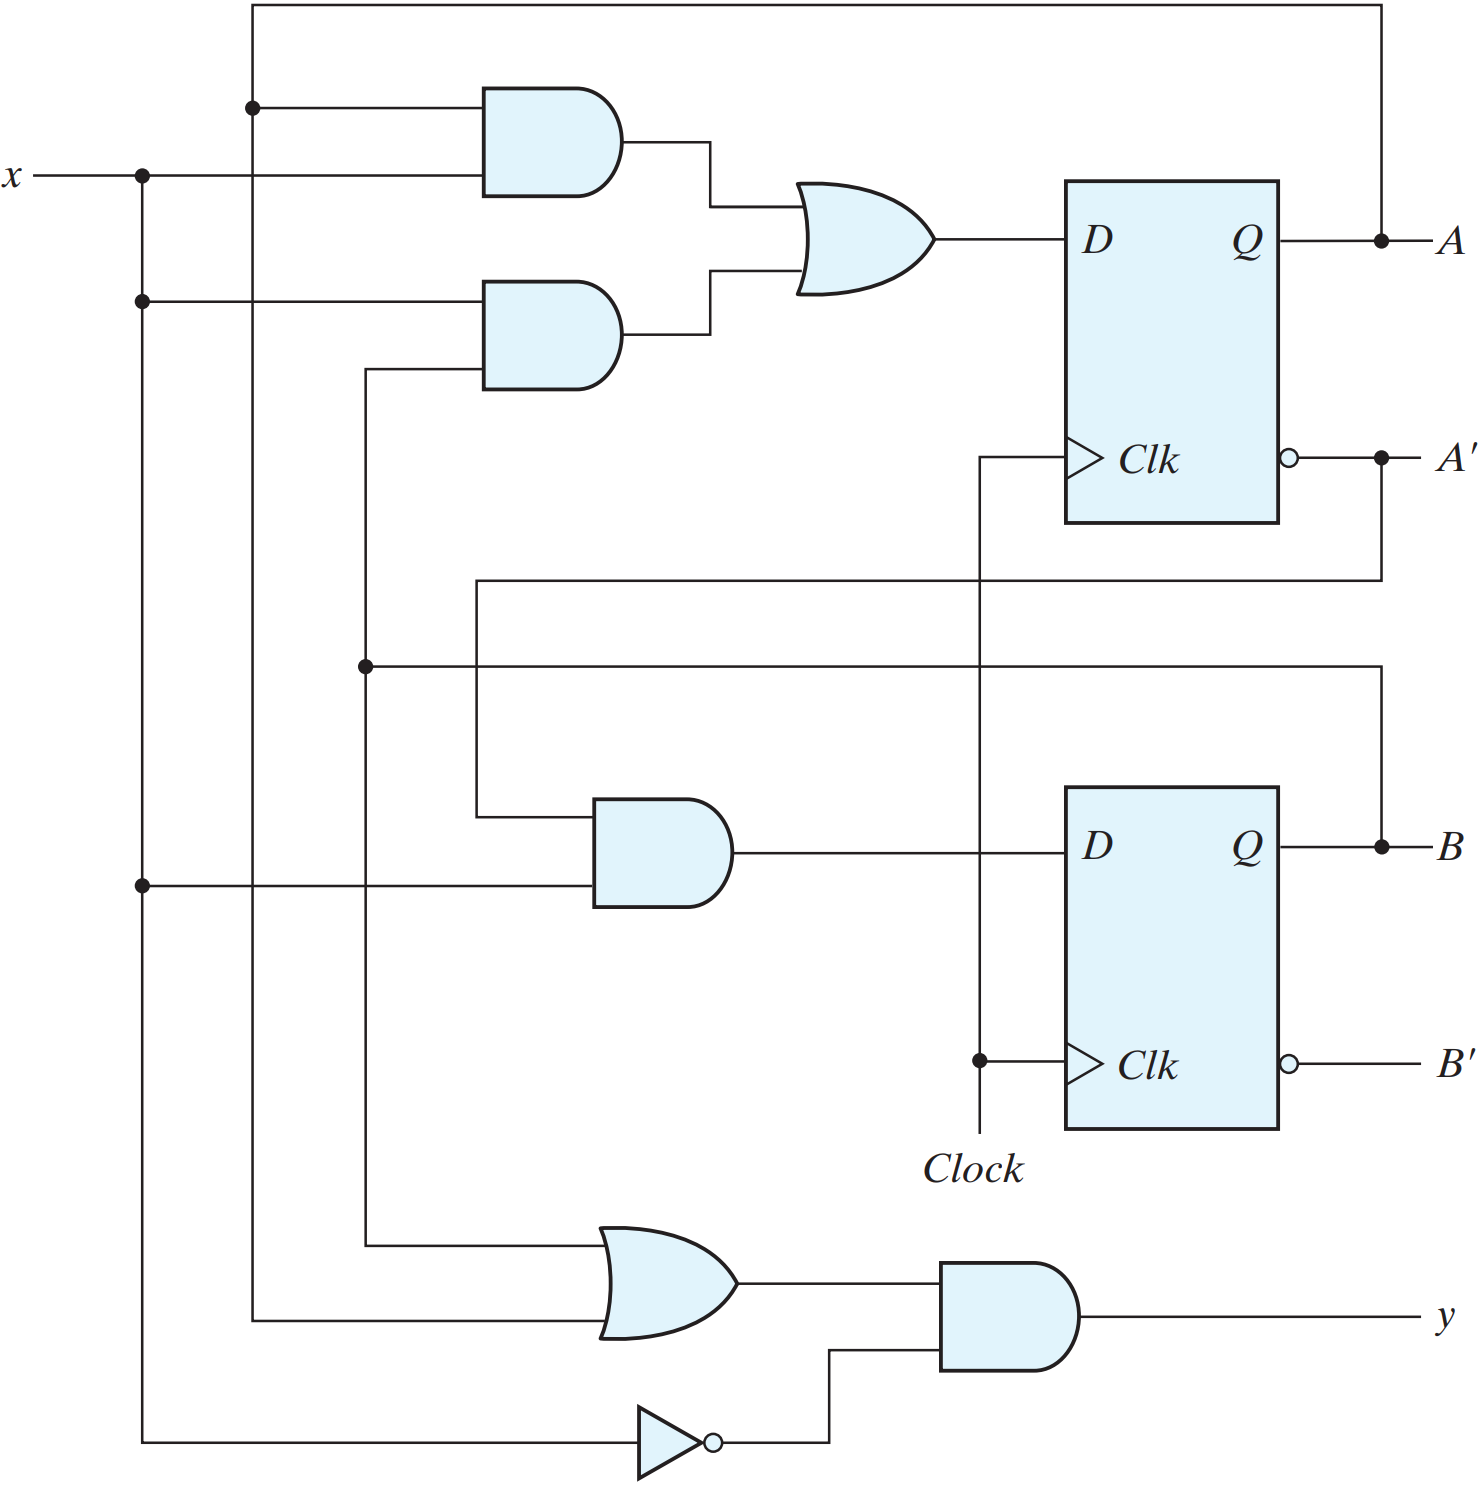
\includegraphics[width=\linewidth]{img/fig-5.15.png}
  \caption{Example of sequential circuit}
  \label{fig:5.15}
\end{figure}
\noindent So the state equations:
\begin{align*}
  A(t + 1) &= Ax + Bx\\
  B(t + 1) &= A'x\\
  y &= (A + B)x'
\end{align*}

\subsection{State Table}
\label{subsec:state-table}

The time sequence of inputs, outputs, and flip-flop states can be enumerated in a \textit{state table} (sometimes called a \textit{transition table}). The state table for the circuit of Fig. 15 is shown in Table 5.2. The table consists of four sections labeled \textit{present state}, \textit{input}, \textit{next state}, and \textit{output}.

\noindent The derivation of a state table requires listing all possible binary combinations of present states and inputs. In general, a sequential circuit with $m$ flip-flops and $n$ inputs needs $2^{m + n}$ rows in the state table.

\vspace*{\fill}
\columnbreak

\begin{figure}[H]
  \centering
  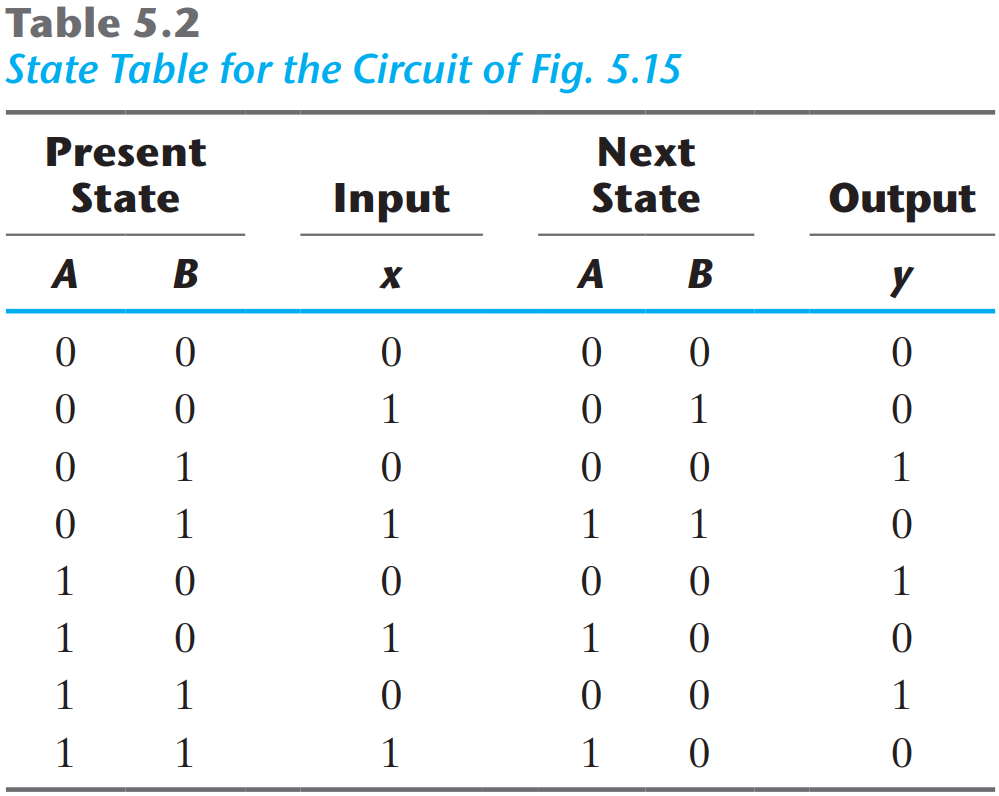
\includegraphics[width=.8\linewidth]{img/table-5.2.png}
  \label{table:5.2}
\end{figure}

It is sometimes convenient to express the state table in a slightly different form having only three sections: \textit{present state}, \textit{next state}, and \textit{output}. The input conditions are enumerated under the next-state and output sections. The state table of Table 5.2 is  repeated in Table 5.3 in this second form.
\begin{figure}[H]
  \centering
  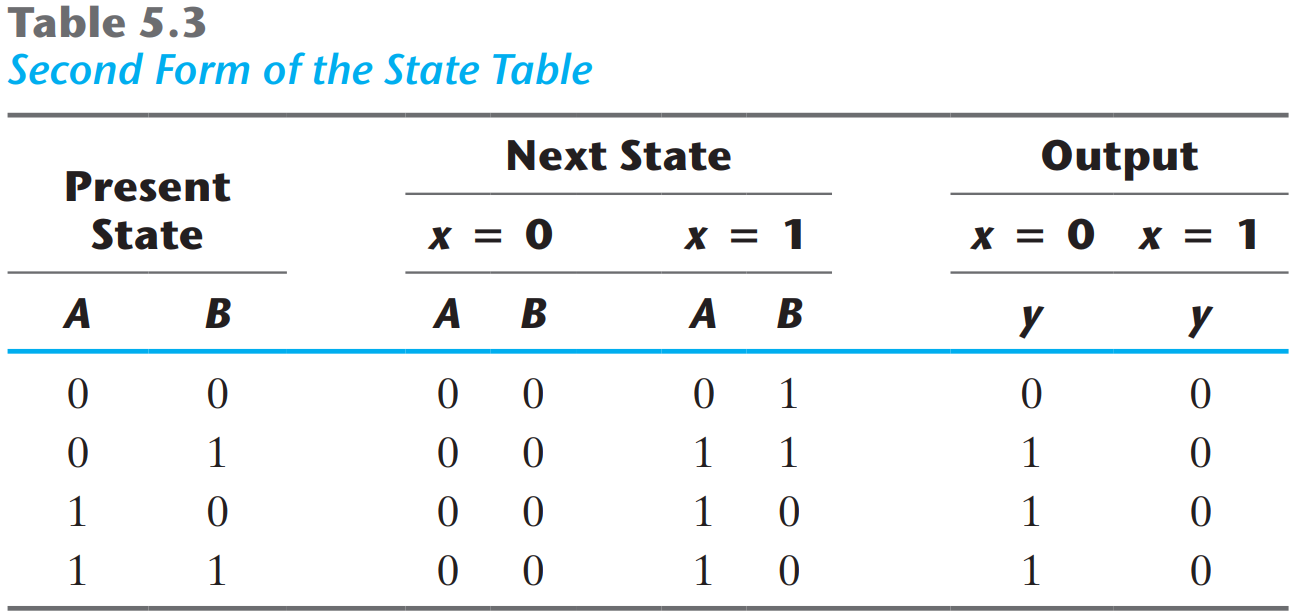
\includegraphics[width=.9\linewidth]{img/table-5.3.png}
  \label{table:5.3}
\end{figure}

\subsection{State Diagram}
\label{subsec:state-diagram}

The information available in a state table can be represented graphically in the form of a state diagram. In this type of diagram, a state is represented by a circle, and the (clock-triggered) transitions between states are indicated by directed lines connecting the circles.

The state diagram of the sequential circuit of Fig. 15 is shown in Fig. 16. The state diagram provides the same information as the state table and is obtained directly from Table 5.2 or Table 5.3. The binary number inside each circle identifies the state of the flip-flops. The directed lines are labeled with two binary numbers separated by a slash. The input value during the present state is labeled first, and the number after the slash gives the output during the \textit{present} state with the given input.
\begin{figure}[H]
  \centering
  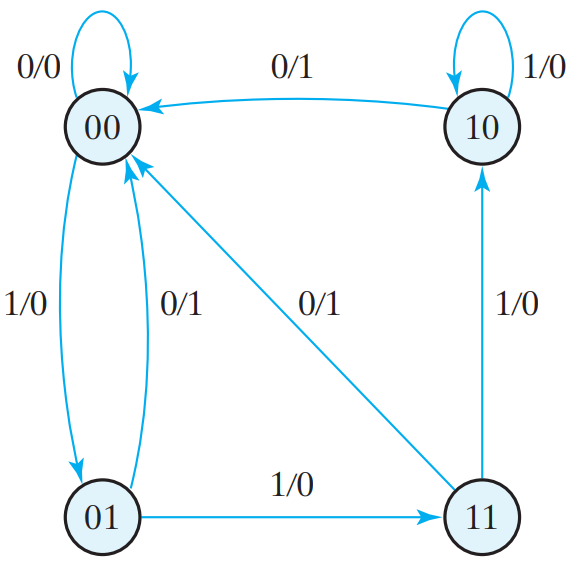
\includegraphics[width=.5\linewidth]{img/fig-5.16.png}
  \caption{State diagram of the circuit of Fig. 15}
  \label{fig:5.16}
\end{figure}

\noindent The steps presented in this example are summarized below:
\begin{center}
  Circuit diagram $\ra$ State Equations $\ra$ State Table $\ra$ State Diagram
\end{center}

\noindent To analyze sequential circuits:
\begin{itemize}
  \item Find Boolean expressions for the outputs of the circuit and the flip-flop inputs.
  \item Use these expressions to fill in the output and flip-flop input columns in the state table.
  \item Finally, use the characteristic equation or characteristic table of the flip-flop to fill in the next state columns.
\end{itemize}
The result of sequential circuit analysis is a state table or a state diagram describing the circuit.

\textit{\textbf{Note:} There are some examples in book that are realted to analysis. Examine them carefully.}

\subsection{Mealy and Moore Models of Finite State Machine}
\label{subsec:mealy-and-moore-models}

\begin{figure}[H]
  \centering
  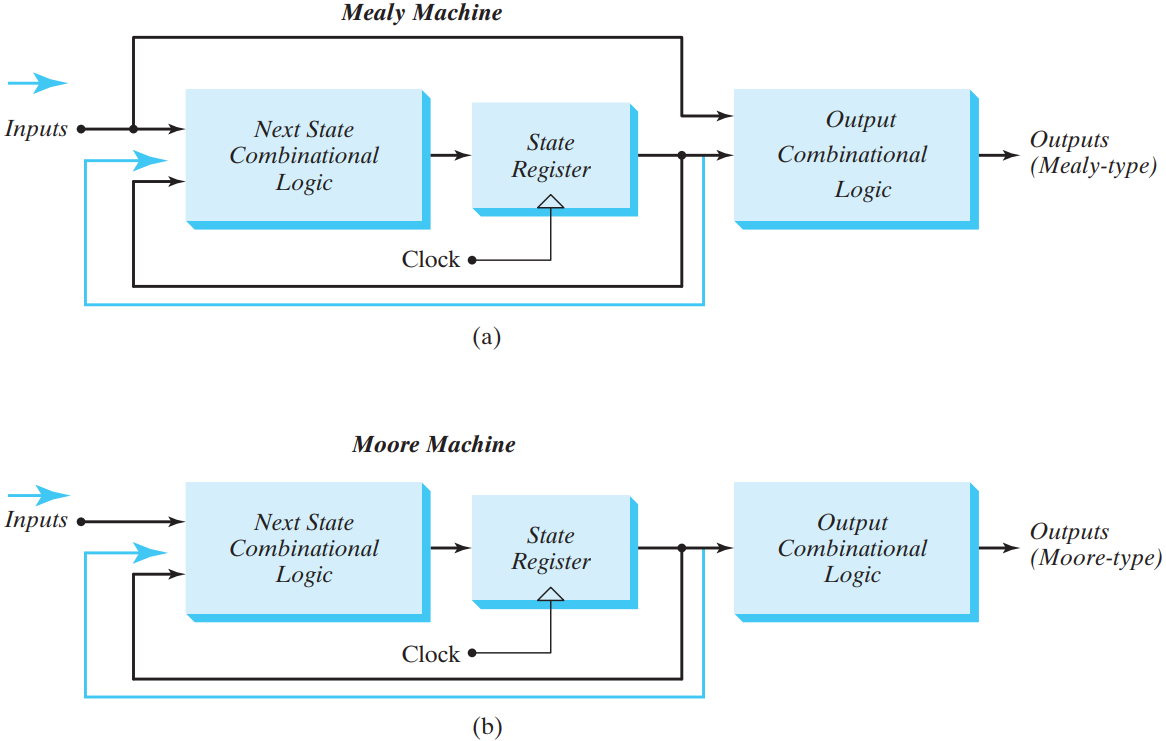
\includegraphics[width=\linewidth]{img/fig-5.21.png}
  \caption{}
  \label{fig:5.21}
\end{figure}

In a Moore model, the outputs of the sequential circuit are synchronized with the  clock, because they depend only on flip-flop outputs, which are synchronized with the clock.

The output of the Mealy machine is the value that is present immediately before the active edge of the clock.

\textbf{Notes:}
\begin{itemize}
  \item The difference between a Mealy and Moore state machine is that ``\textit{the output of a Moore state machine depends on only the state of the machine; the output of a Mealy machine depends on the present state and the inputs to the machine.}
  \item \textit{The edge of a state machine chart represents a transition of the machine between two states.}
  \item \textit{A transition between the states of a finite state machine occurs at the active edge of the synchronizing signal (clock).}
  \item \textit{A finite state machine may have synchronous or asynchronous reset.}
  \item The reason why it is an important practice to implement a reset  signal in a finite state machine is that ``\textit{ Without a reset signal a finite state machine cannot be driven into a known initial state.}''.
  \item \textit{The outputs of a Mealy state machine may depend on the inputs to the machine.}
\end{itemize}

\section{State Reduction and Assignment}
\label{sec:state-reduction-and-assignment}

The goal is to \textit{reduce the number of states while keeping the external input-output requirements}. $2^m$ states need $m$ flip-flops, so reducing the states may reduce flip-flops. In other words, by reducing states, number of flip-flops can also be reduced. If two states are equal, one can be removed.
\begin{quote}
  State Equivalence: ``Two states are said to be equivalent if, for each member of the set of inputs, they give exactly the same output and send the circuit either to the same state or to an equivalent state.''
\end{quote}
\noindent After a state is reduced, state table may need to be reorginazed by new state assignments.

\subsection*{Example}

As an example consider the state diagram (initially, reaching $f$ generates output 1)
\begin{figure}[H]
  \centering
  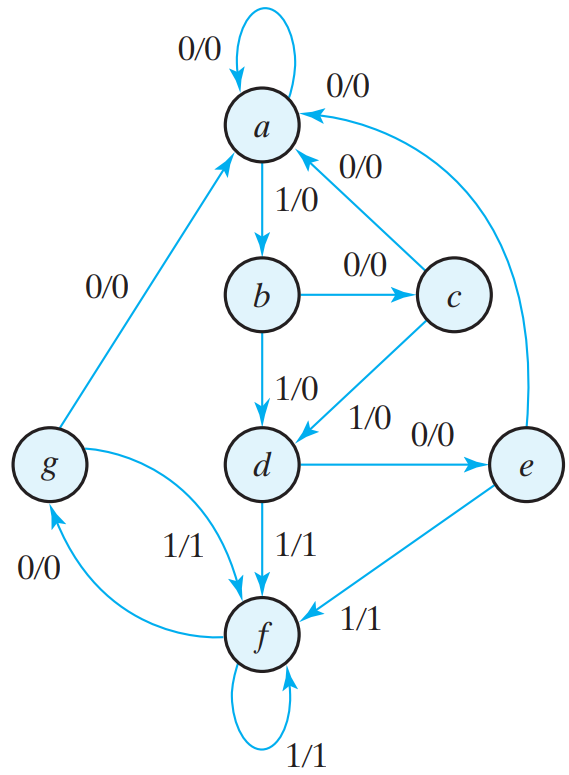
\includegraphics[width=.7\linewidth]{img/fig-5.25.png}
  \caption{A state diagram}
  \label{fig:fig5.25}
\end{figure}

\vspace*{\fill}
\columnbreak

\noindent The state table of the diagram is the following:
\begin{figure}[H]
  \centering
  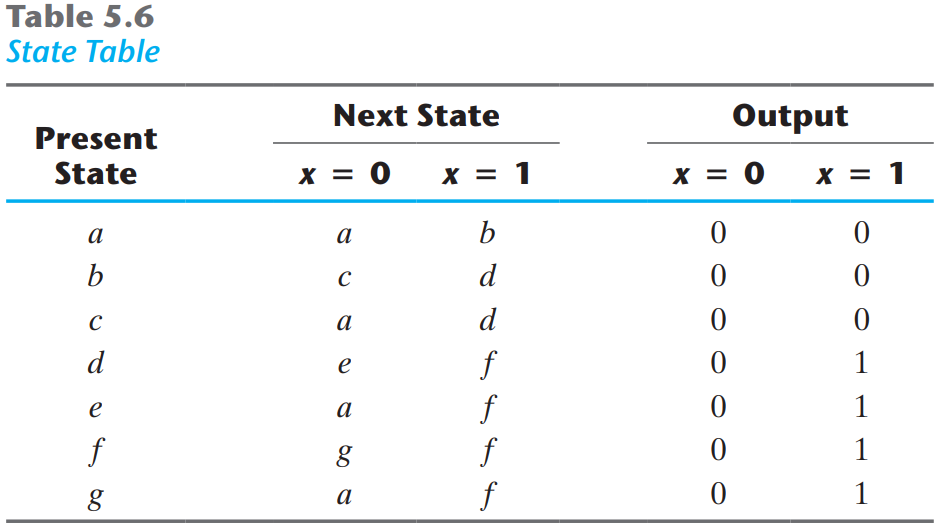
\includegraphics[width=\linewidth]{img/table-5.6.png}
  \label{table:5.6}
\end{figure}

States $e$ and $g$ are equal since for each member of the set of inputs, they give the same output and send the circuit either to the same state or an equivalent state. So one of them can be removed. So, state $g$ is removed and replaced by state $e$:
\begin{figure}[H]
  \centering
  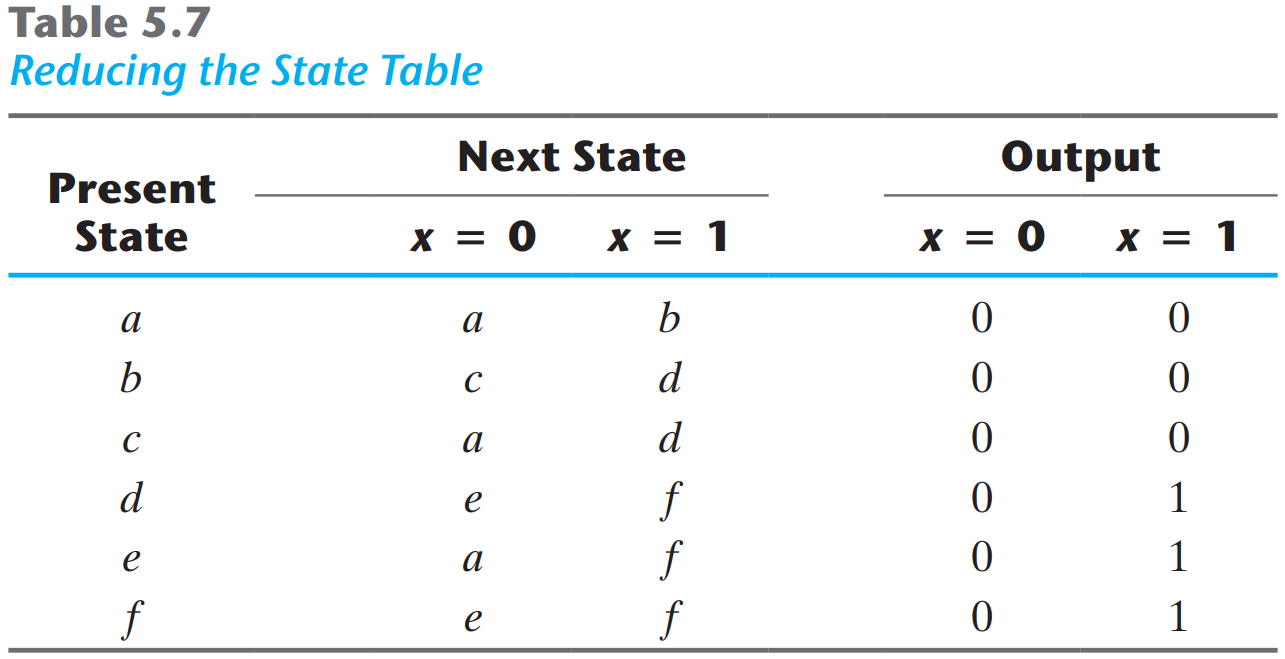
\includegraphics[width=\linewidth]{img/table-5.7.png}
  \label{table:5.7}
\end{figure}
\noindent Notice that, a state equivalence is formed. State $d$ and $f$ are equivalent. So, we can remove $f$ and replaced it with $d$:
\begin{figure}[H]
  \centering
  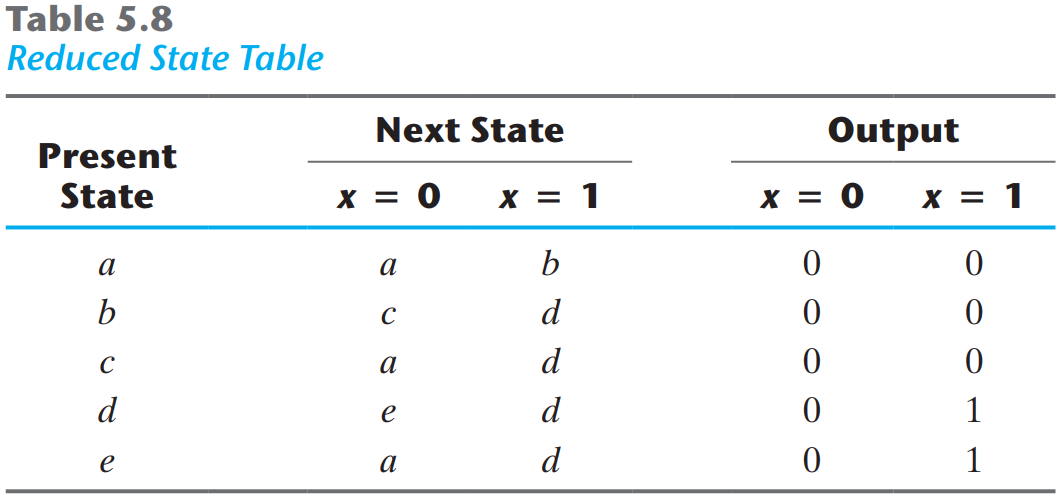
\includegraphics[width=\linewidth]{img/table-5.8.png}
  \label{table:5.8}
\end{figure}


\vspace*{\fill}
\columnbreak

\section{Sequential Circuit Design}
\label{sec:seq-circ-design}

Sequential circuit design is to produce a working circuit for a given description or problem.

\subsection{Excitation Tables}

Excitation table is \textit{a table that lists the required inputs for a given change of state}.
\begin{figure}[H]
  \centering
  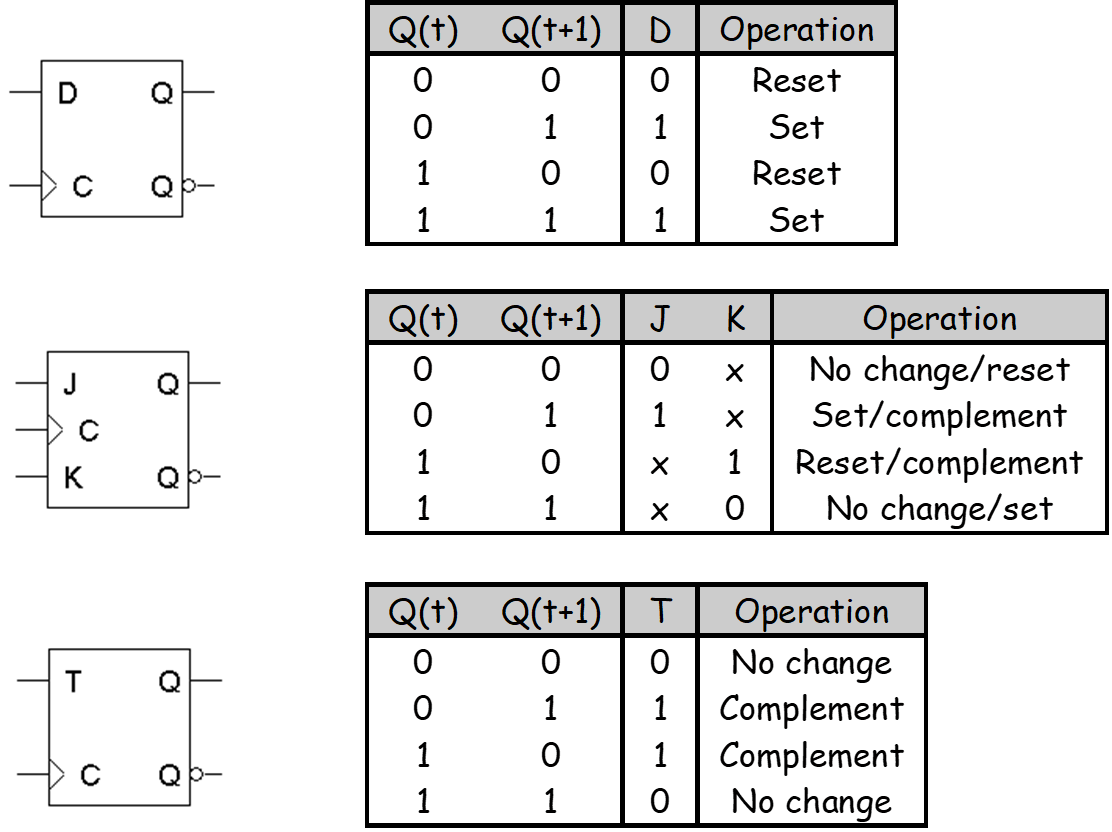
\includegraphics[width=\linewidth]{img/excitation-tables.png}
  \caption{Excitation Tables of Flip-Flops}
  \label{fig:excitation-tables}
\end{figure}

\subsection{Sequential Circuit Design Procedure}
\label{subsec:seq-circ-design-procedure}

\begin{enumerate}[label=Step\ \arabic*:, leftmargin=*]
  \item Make a state table based on the problem statement. The table should show the \textit{present states}, \textit{inputs}, \textit{next states} and \textit{outputs}. (\textit{It may be easier to find a state diagram first, and then convert that to a table.})
  \item Assign binary codes to the states in the state table (if you haven't already). If you have $n$ states, your binary codes will have at least $\lceil \log_2 n \rceil$ digits, and your circuit will have at least $\lceil \log_2 n  \rceil$ flip-flops.
  \item For each flip-flop and each row of your state table, find the flip-flop input values that are needed to generate the next state from the present state. You can use flip-flop excitation tables here.
  \item Find simplified equations for the flip-flop inputs and the outputs.
  \item Build the circuit!
\end{enumerate}

\vspace*{\fill}
\columnbreak

\subsection{Example: Sequence Recognizer}
\label{subsec:example-seq-recozginer}

Consider an example that the sequence recognizer will detect the bit pattern ``1001'' with input $X$ and output $Z$. Note that overlapping bit patterns are also detected. (1001001 will generate 0001001)

\subsubsection{Step 1: State Diagram (and Table)}
\label{subsubsec:step1-state-diagram-table}

\begin{figure}[H]
  \centering
  \begin{minipage}{\linewidth}
    \centering
    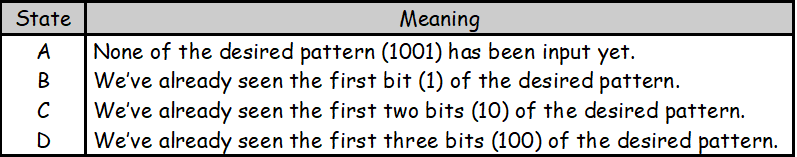
\includegraphics[width=\linewidth]{img/desing-example-table.png}
  \end{minipage}
  \begin{minipage}{\linewidth}
    \centering
    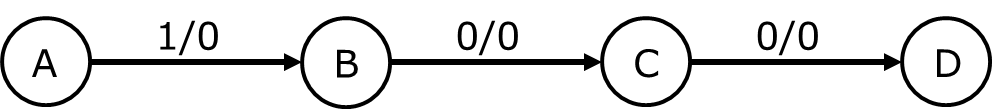
\includegraphics[width=\linewidth]{img/design-example-state-diagram.png}
  \end{minipage}
\end{figure}

What happens if we're in state D (the last three inputs were 100), and the current input is 1?
\begin{figure}[H]
  \centering
  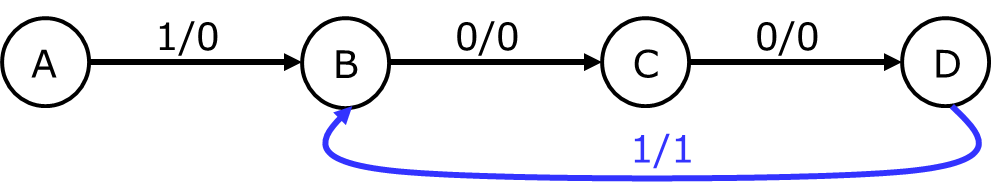
\includegraphics[width=.85\linewidth]{img/design-example-state-diagram-2.png}
\end{figure}

\noindent When we put the other arrows:
\begin{figure}[H]
  \centering
  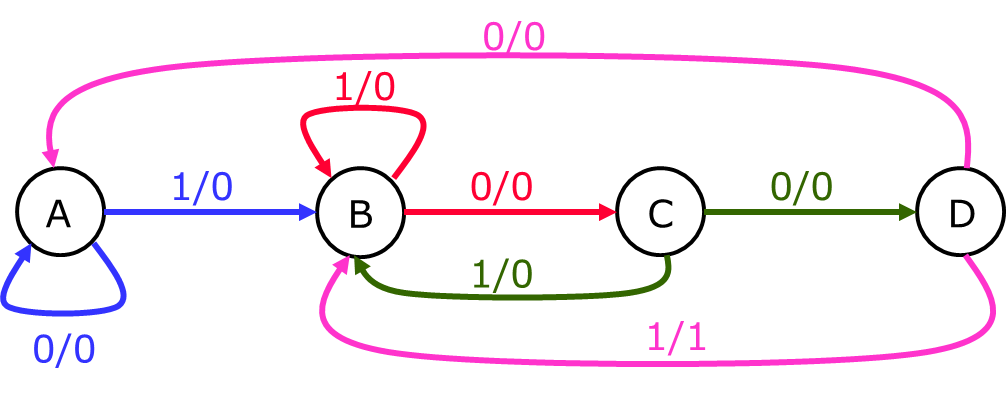
\includegraphics[width=\linewidth]{img/design-example-state-diagram-4.png}
\end{figure}
\noindent Finally, making the state table.
\begin{figure}[H]
  \centering
  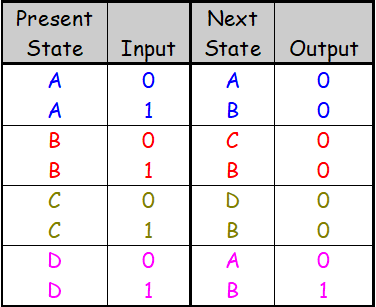
\includegraphics[width=.8\linewidth]{img/desing-example-state-table.png}
\end{figure}

\vspace*{\fill}
\columnbreak

\subsubsection{Step 2: Assigning Binary Codes}
\label{subsubsec:step2-assign-bin-code}

\begin{figure}[H]
  \centering
  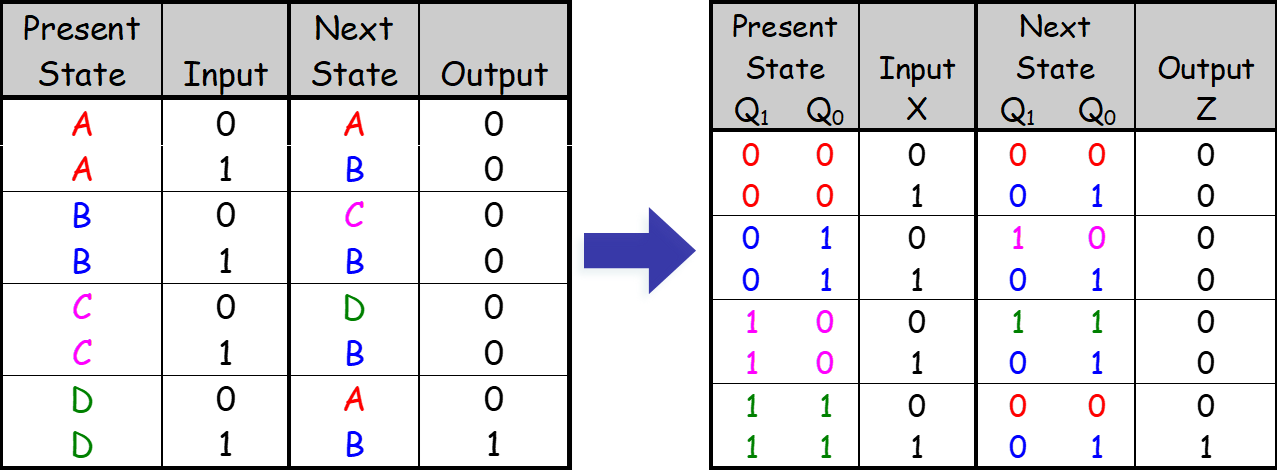
\includegraphics[width=\linewidth]{img/desing-example-state-table-2.png}
\end{figure}

\subsubsection{Step 3: Finding Flip-Flop Inputs}
\label{subsubsec:step3-finding-ff-inputs}

By using excitation table:
\begin{figure}[H]
  \centering
  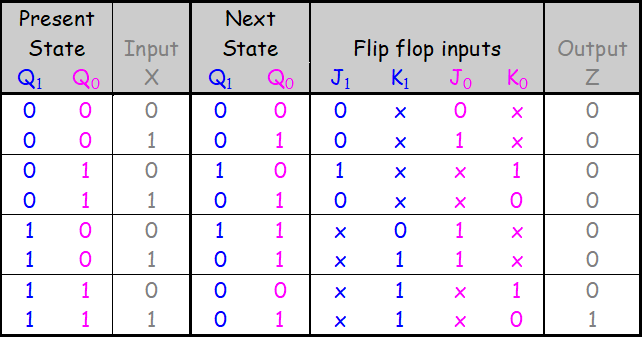
\includegraphics[width=\linewidth]{img/desing-example-state-table-3.png}
\end{figure}

\subsubsection{Step 4: Find Flip-Flop In/Out Equations}
\label{subsubsec:step4-find-ff-io-equations}

\noindent By using K-Maps, find equations for input and output:
\begin{align*}
	J_0 &= X + Q_1\\
	K_0 &= X'\\
  &\\
  J_1 &= X'Q_0\\
	K_1 &= X + Q0\\
  &\\
	Z &= Q_1Q_0X
\end{align*}

\subsubsection{Step 5: Build the Circuit}
\label{subsubsec:step5-build-the-circuit}

Lastly, we use these simplified equations to build the completed circuit.
\begin{figure}[H]
  \centering
  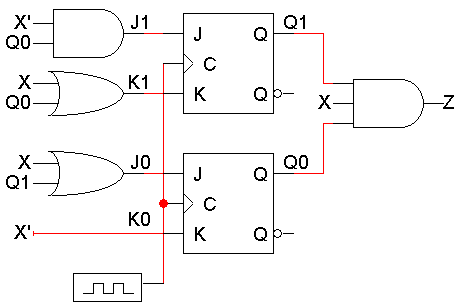
\includegraphics[width=\linewidth]{img/design-example-circuit.png}
\end{figure}

\end{multicols*}

\end{document}
